% Kapitel 2 mit den entsprechenden Unterkapiteln
% Die Unterkapitel können auch in separaten Dateien stehen,
% die dann mit dem \include-Befehl eingebunden werden.
%-------------------------------------------------------------------------------
\chapter{Analyse der Produktfunktionen}

%Dieser Abschnitt stellt die Basis für die Festlegung der Architektur dar. Die
%Festlegung einer geeigneten Architektur geschieht aufgrund der im Pflichtenheft
%analysierten Produktfunktionen und nicht-funktionalen Anforderungen, die
%realisiert werden müssen. Jede betrachtete Funktion wird in einem eigenen
%Unterkapitel dokumentiert.  Fügen Sie bitte so viele Unterkapitel ein, wie
%Produktfunktionen im Pflichtenheft vorhanden sind. Auch die nicht-funktionalen
%Anforderungen sind so weit möglich entsprechend darzustellen.
%
%
%\section{Analyse von Funktionalität <ID aus Pflichtenheft>: <Funktionsname>}
%z.B.: Analyse von Funktionalität /F10/: Automatisches Einlagern
%In diesem Abschnitt wird die im Titel angegebene Produktfunktion sowohl im
%Hinblick auf ihre Verteilung auf die Architektur als auch im Hinblick auf die
%zu ihrer Realisierung nötigen Datenstruktur untersucht.  Zu Beginn die
%Funktionalität kurz beschreiben.  Anschließend erfolgt die Darstellung der
%Realisierung der Funktion als Interaktion von Komponenten des zu entwickelnden
%Systems in einem Sequenzdiagramm. Das Diagramm bitte ebenfalls kurz
%beschreiben.
Im folgenden werden die Funktionen und Qualitätsmerkmale des System auf ihre
Komponentenzugehörigkeit hin geprüft und eingeordnet. Dabei wird auf das
Basis-Konstrukt von Django aufgebaut und die Funktionen bzw. Qualitätsmerkmale
werden in unterschiedliche Kategorien eingeteilt.

Die Funktionen werden den Programmkomponenten zugeordnet. Die Funktionen lassen
sich weiter in den folgenden Gruppen beschreiben:
\begin{description}
	\item[Build-In Django] Eine Funktion die bereits von Django bereit gestellt
	  wird.
	\item[Model einer Django-App] ist in Django für die Klassen und
	  Datenbankstruktur der zugrundeliegenden Datenbank zuständig.
	\item[Klassen bzw. Objectmethode] sind die Klassen bzw. Objekte die in den
	  Models einer Django-App eingeteilt sind.
	\item[Template] ist die allgemeine Beschreibung einer Webseite, die im Falle
	  von Django in einer speziellen Syntax beschrieben wird.
	\item[View im Backend] wird in Django durch die Komponente \textbf{Admin}
	  repräsentiert.
\end{itemize}

%% Aufgaben: 
% Kapitel 1 bearbeiten   %% Marco
\section{Analyse von Funktion F100 (Anmeldung)}
Der Benutzer meldet sich auf dem System unter seinem Benutzernamen an.

Diese Funktion, die lediglich in der Komponente \textbf{View} vorkommt, ist
eine Built-in-Funktion von Django. Innerhalb von Django werden die Benutzer
in einer eigenen Datenstruktur  dargestellt. Diese Klasse muss erweitert werden,
um die zusätzlichen Daten der Benutzer zu speichern. Da Django eine Datenbank
zugrunde liegt, müssen diese weiteren Daten in einer extra Klasse mit Referenz
auf die Benutzer gesetzt werden.

\section{Analyse von Funktion F101 (Anmeldung über LDAP)}
Der Benutzer meldet sich auf dem System über seinen \Gls{GITZ}-Benutzer an.

Diese Funktion wird in einer extra App dargestellt. Die \gls{LDAP}-Anmeldung muss
dabei die normale Anmeldung erweitern und im View evtl. durch eine Checkbox zur
Verfügung gestellt werden. Die zugrundeliegende Datenstruktur wird von \gls{LDAP}
bereit gestellt.

\section{Analyse von Funktion F102 (Anbindung an die Universitätsbibliothek)}
Ein Benutzer mit hinreichenden Rechten verschickt an die Universitätsbibliothek
den Stand der aktuellen Datensätze.

Der zugrunde liegende Datensatz der Dokumente wird von einem, in den
\textbf{Models} gelegenen Befehlssatz in ein Datenformat übersetzt, welches von
der TU Braunschweig Universitätsbibliothek gelesen werden kann. 

\section{Analyse von Funktion F103 (Mailtexte ändern)}
Die Standard-Mails, die vom System an Benutzer verschickt werden, sollen geändert
werden.

Die Mailtexte sind Bestandteil einer veränderbaren, aber nicht großen Tabelle an
Basisinformationen, wie auch andere Einstellungen für die Software. Um die
Informationen bereit zu stellen, muss eine neue Klasse in den \textbf{Models}
erzeugt werden, die alle Informationen für die App bereit stellt.

\section{Analyse von Funktion F201 (Bib\TeX\ import)}
Ein oder mehrere Dokumente werden zum System hinzugefügt. Dafür wählt der
Benutzer den entsprechenden View aus und lädt über einen Upload-Dialog eine
\BibTeX -Datei hoch. Das System analysiert die Datei auf Validität, erzeugt
Objekte aus den Daten, die in eine Datenbank gespeichert werden.

Für die Funktion wird also ein \textbf{View} benötigt, der den Upload bereit
stellt.  Als Basis werden die Dokument-Objekte aus den \textbf{Models} benötigt,
die auch von vielen weiteren Funktionen verwendet werden und die auch über
Django die Datenbankeinträge verwalten.
 % Q10 zusätzlich! %% Theo
\section{Analyse von Funktion F201 (Webinterface-Import)}
\label{f:201}
Der Benutzer, der entsprechende Rechte hat, wählt einen View, der ein Interface
bietet um die Daten für einzelne Dokumente in das System ein zu pflegen. Dafür
wird ihm vom System eine Eingabemaske auf dem View geboten.

Diese Funktion stellt für den Benutzer eine weitere Schnittstelle zur internen
\BibTeX -Verwaltung. Es handelt sich also nur um einen weiteren View zu einer
bestehenden Funktion, weswegen auf eine Grafik verzichtet wird


\section{Analyse von Funktion F202 (Editieren von Dokumenten)}
% Grafik?
Der Benutzer, der entsprechnde Rechte hat, nimmt auf der Detailansicht eines
Dokumentes die Möglichkeit wahr, die Daten Dieses nachträglich zu ändern. Dafür
wählt der die entsprechnde Option und wird vom System auf eine Seite ähnlich der
aus \ref{f:201}\nameref{f:201} mit einer ausgefüllten Maske.

Diese Funktion muss zurest das Dokument auslesen um den View zu erzeugen und
dann die Einträge des Dokumentes entsprechend ändern. Eine solche Veränderung
von den Objekten benötigt lediglich entsprechnende set- und get-Methoden für die
Dokumente und einen entsprechenden View für Django.

\section{Analyse von Funktion F203 (Löschen von Dokumenten)}
Der Administrator, als einziger Benutzer mit den entsprechenden Privilegien,
löscht ein Dokument vollständig aus der Datenbank inkl. der Ausleihhistory.
Diese Aktion wird über einen View im Backend erledigt, der dort bereit steht.

Benötigt wird für Django ein entsprechender View im Backend, der die Möglichkeit
bietet die eingetragenen Dokumente im Backend ein zu sehen. Weiter wird die
zugrundeliegende Funktion der Löschung von Objekten aus der Datenbank benötigt,
die in Django bereits build-in ist. Aufgrund des nicht sehr komplexen
Funktionsaufbaus wurde auf eine Funktion verzichtet.

\section{Analyse von Funktion F210 (Generelle Suche)}
Der Benutzer gibt in eine Suchmaske einen oder mehrere Begriffe ein, um seine
Suche zu spezifizieren. Nach der Bestätigung der Eingabe gibt das System
entsprechende Treffer dem Benutzer in einer Liste zurück.

Die zugrundeliegenden Funktionen der Objekt-Suche nach bestimmten Parametern
wird bereits durch Django bereit gestellt. Der Such-View arbeitet auf dabei auf
einer Funktion die für die Dokumentfunktionen arbeitet.

Da diese Suche mit der weitläufig bekannten Google-Suche vergleichbar ist wird
auf eine Grafik verzichtet.
 %% Theo
\section{Analyse von Funktion F210 (Generelle Suche)}
Diese Funktion ist eine Build-In Funktion von Django. Das gesuchte Wort wird einfach mithilfe einer Search-Query innerhalb der Datenbank gesucht und ausgegeben. 

\section{Analyse von Funktion F211 (Suche mit erweiterten Ausdrücken)}
Auch diese Suche wird von Django mithilfe von mehreren Querysets bereitgestellt und ist daher bereits eine Built-In Funktion.

\section{Analyse von Funktion 212 (erweiterte Suche)
Im FrontEnd werden die bestätigten Parameter (aus der Maske für die erweiterte Suche) den dazu passenden Built-In Querysets im System übergeben. 

\section{Analyse von Funktion 213 (Suche mit regulären Ausdrücken)
Diese Funktion muss in einer extra App dargestellt werden, wo genau bestimmt wird, welche aus der FrontEnd ermittelten Zeichenfolgen in der Suchanfrage bestimmte Querysets auslösen.

\section{Analyse von Funktion 214 (Sortierung der Suche)
Auch diese Funktion muss in einer extra App dargestellt werden. Das vorläufige Ergebnis aus einer Suchanfrage wird tabellarisch angezeigt, dessen Spalten aber interaktiv sind: Die Spaltennamen lösen system-intern Funktionen aus, die aus Build-In Querysets bestehen, die genau bestimmen, wie die Ergebnisse dargestellt werden sollen (in diesem Fall alphabetisch aufwärts/abwärts). 



  %% Johann
\section{Analyse von Funktion F220: Ausleihe}
\label{f:220}
Ein oder mehrere Dokumente werden von einem Benutzer ausgeliehen. Dabei wählt 
der Benutzer das gewünschte Dokument aus und das System muss in der Datenbank 
nachprüfen, ob dieses derzeit ausleihbar ist. Wenn dies der Fall sein sollte, 
wird dem Benutzer dieses Buch zugewiesen. Dies erfolgt durch zwei 
Built-In-Funktionen von \gls{glos:django}, mit dessen Hilfe die Datenbank 
erweitert bzw.\ ein Datensatz geupdatet werden kann. Es gehört zum 
\textbf{View}-Komponent im Zusammenhang zur \textbf{DB}.

Das Sequenzdiagramm ist strukturell das selbe wie Abb.\ \ref{fig:221}. Es muss 
nur keine Eingabe von \gls{glos:ext}n getätigt werden. Daher entfallen die 
Schritte 1.1 und 1.2. 

\section{Analyse von Funktion F221: Ausleihe an Externe}
\label{f:221}
Die Ausleihe an \gls{glos:ext} ist ähnlich gestaltet wie in \ref{f:220} 
\nameref{f:220} und gehört ebenfalls dem \textbf{View}-Komponent mit 
\textbf{DB}-Einflüssen. Es existiert lediglich der Zusatz, dass der Benutzer 
einen \gls{glos:ext}n als eigentlichen Ausleiher angibt. Dafür wird beim 
Entleihen die Möglichkeit gegeben, Daten über den \gls{glos:ext}n anzugeben, 
dessen Daten dann gespeichert und beim Entleihen vermerkt werden. Auch hierbei 
wird eine Built-In-Funktion zum Erweitern der Datenbank genutzt.

Das Sequenzdiagramm der Abb. \ref{fig:221} ist nur der Hauptteil. Vorher müsste 
erst eine Suchanfrage getätigt werden (wie in Abb.\ \ref{fig:F-A}) bzw.\ eine 
Überprüfung, ob das gewünschte Dokument derzeit vorhanden ist. Außerdem sei 
erwähnt, dass nach jedem Schritt, falls ein Fehler aufgetreten sein sollte, eine 
Fehlermeldung ausgegeben wird.

\begin{figure}
\begin{center}
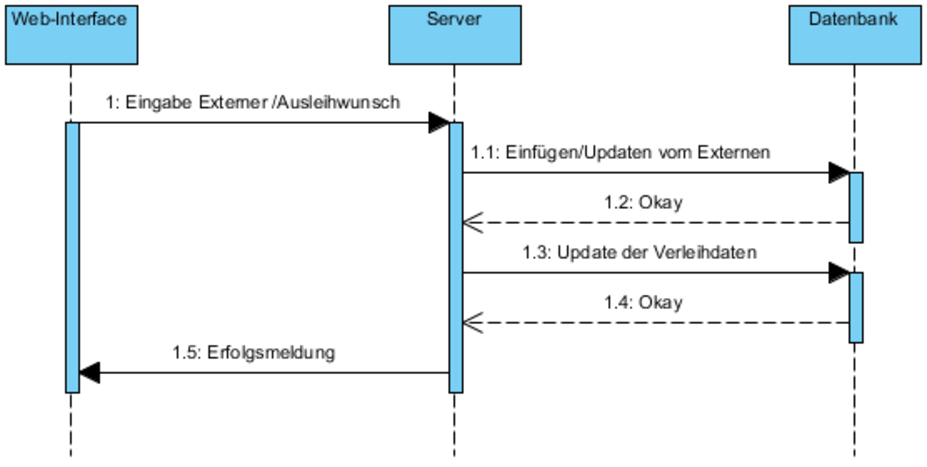
\includegraphics[width=0.8\linewidth]{bilder/Seq-Ausleihe.pdf}
\caption{Sequenzdiagramm für Ausleihe an Externe}
\label{fig:221}
\end{center}
\end{figure}

\section{Analyse von Funktion F222: Ausleihe übertragen}
\label{f:222}
Ein Dokument wechselt den Ausleihenden. Dabei muss ein Benutzer $A$ ein von ihm 
ausgeliehenes Dokument auswählen und einem anderen Benutzer $B$ übertragen. 
Alternativ kann Benutzer $B$ auch eintragen, dass er sich ein Dokument von 
Benutzer $A$ geholt hat, das Dokument also jetzt bei ihm zu finden ist. Das 
System vermerkt dieses Austausch dann in der Datenbank mittels einer 
Built-In-Funktion von \gls{glos:django}. Auch diese gehört zur 
\textbf{View}-Komponente mit Zugriff auf die \textbf{DB}.

Auch dieses Sequenzdiagramm ist strukturgleich mit Abb.\ \ref{fig:221}. Bei 
dieser Funktion muss vorher allerdings geprüft werden, ob das Dokument wirklich 
ausgeliehen ist (auch nur eine Suchanfrage wie in Abb.\ \ref{fig:F-A}). Außerdem 
entfällt wieder die Eingabe von \gls{glos:ext}n (Schritte 1.1 und 1.2).

\section{Analyse von Funktion F223: Ausleihe zurückgeben}
\label{f:223}
Ein Benutzer braucht ein Dokument nicht mehr und gibt es in den Bestand der 
Bibliothek zurück. Auch hierfür muss der Benutzer als Entleiher des Dokumentes 
eingetragen sein. Wenn dies der Fall sein sollte, kann er \emph{zurückgeben} 
wählen und das Dokument wird auch im Datensatz mittels Built-In-Funktionen von 
\gls{glos:django} mit dem Status 0 versehen. Die Funktion ist dem \textbf{View} 
zugeordnet, benötigt aber auch die \textbf{DB}.

Wieder ist die Struktur wie bei Abb. \ref{fig:221} vorzufinden. Hierbei muss 
vorher geprüft werden, ob der Benutzer auch wirklich das Dokument ausgeliehen 
hat (Suchanfrage nach Abb.\ \ref{fig:F-A}. Die Schritte 1.1 und 1.2 zur 
\gls{glos:ext}nausgabe wird wieder weggelassen.

\section{Analyse von Funktion F224: Ausleihe vermisst melden}
\label{f:224}
Das Dokument befindet sich nicht mehr an dem laut Datenbank befindlichen Ort. 
Dann kann ein Benutzer ein Dokument auf der Dokumentenansicht als 
\emph{vermisst} melden und dieses wird in der Datenbank mittels Statusänderung 
vermerkt. Dazu wird eine E-Mail an alle Benutzer verschickt oder alternativ eine
Meldung auf der Homepage angezeigt. Hierfür stellt \gls{glos:django} wieder 
Built-In-Funktionen bereit. Das Ganze gehört dann zu \textbf{View} und 
\textbf{DB}.

Das dazugehörige Sequenzdiagramm ist Abb.\ \ref{fig:224}.
\begin{figure}
\begin{center}
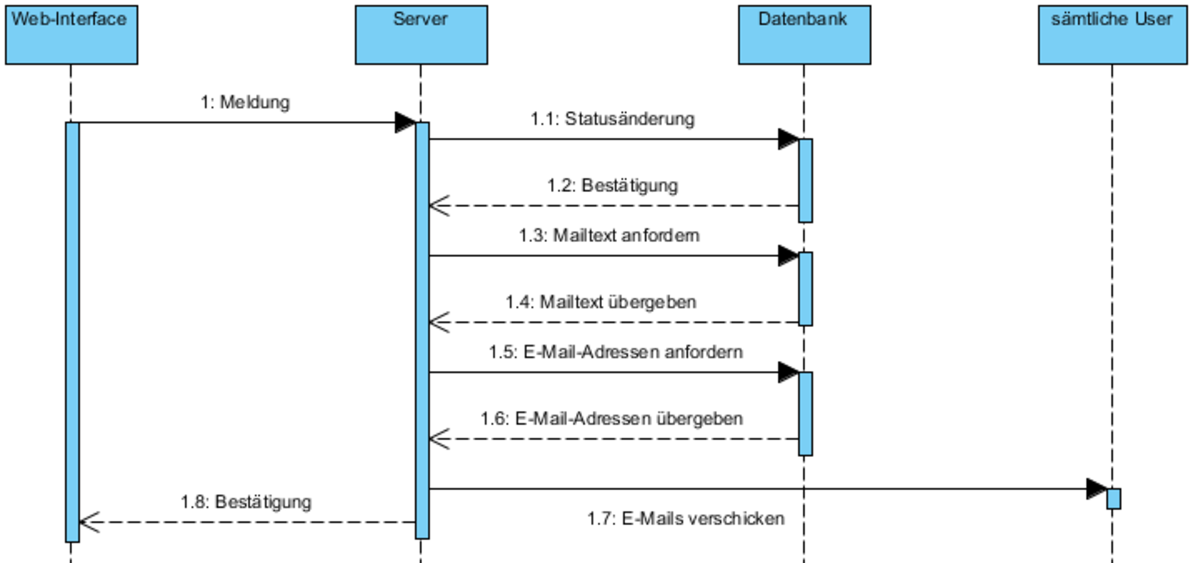
\includegraphics[width=0.8\linewidth]{bilder/Seq-Vermisst.pdf}
\caption{Sequenzdiagramm für eine Vermisstmeldung}
\label{fig:224}
\end{center}
\end{figure}

\section{Analyse von Funktion F225: Ausleihe verloren melden}
\label{f:225}
Das Dokument ist auch nach einer Vermisstenmeldung nicht wieder aufgetaucht. 
Dann ist ein Bibliothekar berechtigt, es als \emph{verloren gegangen} 
einzustufen. Das Dokument bekommt den entsprechenden Status und wird demnächst 
bei weiteren Suchanfragen ausgeschlossen. Dies erfolgt wieder innerhalb der 
\textbf{View}- und \textbf{DB}-Komponenten durch eine Built-In-Funktion von 
\gls{glos:django}.

Das gewünschte Sequenzdiagramm ist strukturell gleich dem von Abb.\ 
\ref{fig:224}. Dabei muss nur vorher geprüft werden, ob der Nutzer die 
entsprechenden Rechte besitzt (Abb.\ \ref{fig:F-A}), und Schritt 1.3 bis 1.7 
entfällt, da keine E-Mails verschickt werden.
 %% Stephan
\section{Analyse von Funktion F226: Ausleihfrist abgelaufen}
Falls die Leihdauer eines Dokumentes abgelaufen ist, wird der Mailtext aus der 
Datenbank abgerufen und an die E-Mail Adressen der beiden Entleiher(Bürge/Entleiher) gesendet.

Hierfür muss eine neue App erstellt werden, welche alle benötigten Informationen enthält bzw. sich aus der Datenbank holt, um diese Funktion zu bewerkstelligen.
Diese Funktion gehört zur Komponente \textbf{Models}, natürlich in Interaktion mit \textbf{DB}

\section{Analyse von Funktion F227: Ausleihhistory}
Die Ausleihhistory ist eine Liste von Personen, welche bereits ein bestimmes Buch ausgeliehen hatten bzw. immer noch haben.
Es wird ein Filter über die Dokument-Objekte gelegt, damit nur bestimmte bzw. die gewünschten Dokumente und deren bisherige Ausleiher ausgegeben werden. Diese so erhaltenen Daten müssen nun noch durch ein Frontend-View an geigneter Stelle der Web-Seite angezeigt werden.
Diese Funktion ist eine Built-In-Funktion von Django und wird über \textbf{View} benutzt. Da die Informationen wiederrum nur in der Datenbank liegen, muss diese Komponente bei jeder Anfrage auf \textbf{DB} zugreifen.

\section{Analyse von Funktion F228: Derzeitiger Leihender}
Die Funktion Derzeitiger Leihender gibt die Person aus, welche grad ein bestimmes Buch ausgeliehen hat.
Da in Django die User durch eine eigene Klasse dargestellt werden, muss diese Klasse auf die Rechte des momentan angemeldeten Benutzers überprüft werden. Falls diese Rechte ausreichend sind, wird wiederum durch ein Queryset+Filter die jeweilige Literatur und der dazugehörige Leihende durch einen View ausgegeben.
Auch diese Funktion benutzt die Komponente \textbf{View} in Zusammenhang mit \textbf{DB} (siehe auch F227}.


\section{Analyse von Funktion F229: Entleihliste}
Wenn der Benutzer angemeldet ist, ist er im Stande, sich alle seine momentan entliehene Dokumente als Liste anzeigen zu lassen.
  
 %% Jörn
\section{Analyse von Funktion F230(\BibTex-Export)}
Die für diesen Export nötigen Informationen sind vollständig in der Datenbank enthalten und müssen mit Django ermittelt werden. Die so erhaltenen Daten werden dem Benutzer in einer View im \BibTex-Format zum Kopieren angezeigt.

\section{Analyse von Funktion F231(Universitätsbibliothek-Export)}
Diese Funktion muss in einer extra App dargestellt werden. Die für diesen Export nötigen Informationen sind vollständig in der Datenbanken enthalten und müssen mittels einer direkten Datenbankabfrage ermittelt werden. Diese Daten werden durch eine Funktion in das richtige Format gebracht und in einem vom Benutzer vorher gewählten Dateipfad in einer .alg-Datei gespeichert. Dieses Sequenzdiagramm ist strukturell genauso wie das für den BibTex-Export, nur das auf eine andere Weise ausgegeben wird. Deswegen wird dies hier weggelassen.

\section{Analyse von Funktion F300(Benutzerverwaltung)}
Alle Informationen zu den Benutzern werden in einer Datenbank gespeichert. Änderungen an bestehenden Benutzern und das Hinzufügen neuer Benutzer wird durch ein Webformular von einem Benutzer mit ausreichenden Rechte eingeleitet. Mithilfe von Django werden die Informationen aus dem Formular gelesen und alle Änderungen in der Datenbank eingetragen. Das Sequenzdiagramm ist trivial, da nur einfach Frage/Antwort-Vorgänge stattfinden.

\section{Analyse von Funktion F301(Rechtezuweisung für Rollen)}
Die Rechte einer Rolle werden in einer eigenen Tabelle der Datenbank gespeichert. Ein Benutzer mit ausreichenden Rechten kann über ein Webformular Änderungen eingeben. Diese Änderungen werden mithilfe von Django aus dem Webformular ausgelesen und in der Tabelle der Datenbank gespeichert. Das Sequenzdiagramm ist trivial, da nur einfach Frage/Antwort-Vorgänge stattfinden.

\section{Analyse von Funktion F302(Benutzer Rolle(n) zuweisen)}
Die Rollen eines Benutzer werden in einer speziellen Tabelle in der Datenbank gespeichert. Ein Benutzer mit ausreichenden Rechten kann über ein Webformular Änderungen eingeben. Diese Änderungen werden mithilfe von Django aus dem Formular ausgelesen und in der entsprechenden Datenbank gespeichert. Das Sequenzdiagramm ist trivial, da nur einfach Frage/Antwort-Vorgänge stattfinden.
 %% Markus

\section{Analyse von Qualitätsmerkmal /Q10/ (Sicherheit der Anmeldung)}
Die Verschlüsselung der Anmeldung wird von Django bereit gestellt und ist daher
bereits eine Build-In-Funktion. 
\section{Analyse von Qualitätsmerkmal /Q11/ (SQL-Injections vermeiden)}

SQL-Statements werden ausschließlich durch Übergabe von Parametern an 
Funktionen von Django ausgeführt. SQL-Injections sind in Django durch 
integriertes Escaping von SQL-Syntax nicht möglich. Nur wenn RAW-SQL 
ausgeführt werden soll, oder aber an die Funktion .extra von Django 
übergeben werden soll, ist eigenes Escaping notwendig.

\section{Analyse von Qualitätsmerkmal /Q20/ (Layoutstruktur)}

Die Templates für Django müssen so angepasst werden, dass sie dem
\Gls{glos:copdes}  der TU Braunschweig entsprechen. Dies wird durch Verwendung
ensprechender Grafiken, Cascading-Stylesheets, Webseitenstruktur und weiteren
Mitteln erreicht.


\section{Analyse von Qualitätsmerkmal /Q21/ (Klare Struktur)}

Die Stylesheets für die Templates von Django sowie die Templates selber
müssen so konstruiert werden, dass der auf der Webseite dargestellte 
Inhalt übersichtlich ist. Menüführung soll ebenfalls ohne Verschachtelung
möglich sein. Ein entsprechendes Design muss vorher entworfen werden.


\section{Analyse von Qualitätsmerkmal /Q22/ (Suche)}

Verwendet wird die in Django bereits implementierte Suche. Diese Suche ist ohne
große Anpassungen bereits intuitiv und einfach nutzbar.


\section{Analyse von Qualitätsmerkmal /Q30/ (Zeichenketten)} 

Die Bearbeitung von Zeichenketten als \Gls{glos:unicode} wird bereits von der benutzten
Datenbank \Gls{glos:sqlite} erfordert, welche nur \Gls{glos:unicode}-codierte Zeichenketten benutzt.


\section{Analyse von Qualitätsmerkmal /Q31/ (Löschen von Dokumenten)} 

Löschen von Dokumenten ist mit Django möglich. Intern muss verhindert werden,
dass andere Nutzer als Administratoren löschen dürfen.
 %% Philipp
